% Introducción
En el siguiente trabajo, desarrollaremos un lenguaje de programación para la materia \Materia{}.
Antes de comenzar propiamente con la definición formal e implementación del mismo, lo correcto es presentar los objetivos que nos hemos impuesto para la creación del lenguaje, y las motivaciones que nos han impulsado al desarrollo de este proyecto.
Por lo tanto, la siguiente sección introducirá al lector los distintos aspectos que influyeron la formación del lenguaje, y justificaron la realización de este trabajo.

\section{Motivación}

En la materia \Materia{}, durante varios años, se ha utilizado un pseudocódigo para la enseñanza de los distintos conceptos que se estudian en la misma.
Debido a esto, el lenguaje que diseñamos (basado en este pseudocódigo) tendrá un fin didáctico, y busca ser otra fuente de aprendizaje para auxiliar el dictado de la asignatura.
Los ejes principales de la materia consisten en el análisis de algoritmos, la definición de tipos abstractos de datos, y la comprensión de diversas técnicas de programación.

El objetivo del pseudocódigo es poder introducir a los estudiantes a nuevos conceptos y fomentar buenas prácticas de programación.
Se utiliza para describir de forma precisa principios operacionales de los distintos algoritmos estudiados en la materia.
Típicamente, se omiten detalles esenciales para la implementación de los algoritmos para favorecer el entendimiento de los mismos.
No existe ningún estándar para la sintaxis o semántica del pseudocódigo, por lo que un programa en este pseudo-lenguaje  no es ejecutable en el sentido que no puede ser traducido a una serie de instrucciones máquina.

Nuestra meta final con este proyecto, es poder tomar la totalidad de los fragmentos de pseudocódigo que se encuentran dispersos en los diversos contenidos de la materia, y transformarlos en un lenguaje completamente implementado, con todo lo que esto implica.
Obviamente, nuestro principal desafío para cumplir nuestra tarea, es poder resolver las distintas ambigüedades y la falta de especificación que el actual pseudocódigo presenta.

\subsection{Objetivos de la Asignatura}

Durante el desarrollo de la materia, se pretende que el alumno adquiera diversos conceptos relacionados con los distintos temas estudiados en la asignatura.
Algunos de los mismos son listados a continuación:
\begin{itemize}
    \item Capacidad para comprender y describir el problema que resuelve un algoritmo (el \textit{qué}), y diferenciarlo de la manera en que lo resuelve (el \textit{cómo}).
    \item Suficiencia para analizar algoritmos, compararlos según su eficiencia en tiempo de ejecución y en espacio de almacenamiento.
    \item Hábito de identificar abstracciones relevantes al abordar un problema computacional, y aptitud para la especificación e implementación de las mismas.
    \item Familiaridad con técnicas de diseño de algoritmos de uso frecuente, y comprensión de diversos algoritmos conocidos.
    \item Contacto con la programación (principalmente en el lenguaje \C{}) de algoritmos y estructura de datos.
    \item Aptitud para la utilización de diversos niveles de abstracción y adaptación a distintos lenguajes de programación.
\end{itemize}

\subsection{Programa de la Asignatura}

El contenido de la materia se puede dividir en tres unidades.
En cada una de estas, se introducen nuevos conceptos que luego se reflejan en diversos fragmentos de pseudocódigo empleados para facilitar la comprensión de los mismos.
En el diseño del futuro lenguaje, se deberán tener en cuenta todas estas cuestiones para poder crear una herramienta útil para complementar la enseñanza de la asignatura.

\subsubsection{Análisis de Algoritmos}

La primer unidad de la materia, se basa en el análisis de algoritmos.
Inicialmente, se estudian distintas maneras de ordenar arreglos utilizando diversas técnicas, como \textit{ordenación por selección}, \textit{ordenación por inserción}, \textit{ordenación por intercalación}, \textit{ordenación rápida}, entra otras.
Con estos contenidos básicos presentes, se enseña al alumno a contar operaciones de un programa, introduciendo de esta forma los conceptos de \textit{orden} y \textit{jerarquía} sobre la complejidad de un algoritmo.
Para terminar, se introducen las recurrencias \textit{divide y vencerás}, y se presentan otros algoritmos como la \textit{búsqueda lineal}, y la \textit{búsqueda binaria}.

\subsubsection{Estructura de Datos}

La segunda parte de la materia, presenta la noción de estructuras de datos.
Se describen a los \textit{tipos concretos} como un concepto relativo a un lenguaje de programación, donde se estudian elementos como los arreglos, las listas, los registros, y los tipos enumerados.
Mientras, los \textit{tipos abstractos} se presentan como una idea asociada a un problema que se quiere resolver.
Se describe la diferencia entre la \textit{especificación}, y la \textit{implementación} de los mismos, y se enseña la importancia de la elección adecuada para estos.
Se examinan diseños distintos para varios de los diversos \textit{TAD's}, como el \textit{contador}, la \textit{pila}, la \textit{cola}, y el \textit{árbol}, junto con la eficiencia en tiempo o espacio de sus distintas operaciones.
Además, se introduce el concepto de \textit{manejo dinámico de memoria} de un programa mediante el uso de punteros.

\subsubsection{Algoritmos Avanzados}

La última unidad, presenta distintas estrategias conocidas para la resolución de problemas algorítmicos.
Se introduce el esquema general de los \textit{algoritmos voraces}, y se enseñan diversos algoritmos que se basan en esta idea como el de \textit{Dijkstra}, \textit{Prim}, y \textit{Kruskal}.
También se introduce al concepto de \textit{backtracking}, resolviendo los problemas de la \textit{moneda}, y la \textit{mochila}, entre otros.
Luego, se ve \textit{programación dinámica} donde se visitan problemas previos, además de ver nuevos conceptos como el algoritmo de \textit{Floyd}.
Un último tema que se enseña en la materia, es la recorrida de grafos, y las distintas variantes para realizar la misma.

\section{Características del Lenguaje}

Una vez detallados los fundamentos en los que se basa el lenguaje, es hora de describir sus características más importantes.
\Lenguaje{} es una formalización del pseudocódigo utilizado en la materia \Materia{}, por lo que está diseñado para enseñar conceptos fundamentales de forma clara y natural.
Es un lenguaje imperativo similar a \Pascal{}.
Este último fue diseñado por \textit{Niklaus Wirth} cerca de 1970~\cite{Pascal}.
Algunos elementos básicos que comparten son:
\begin{itemize}
    \item Una sintaxis verbosa, pero fácil de leer.
    \item Un tipado fuerte para las expresiones.
    \item Un formato estructurado del código.
\end{itemize}

Al solo contar con una definición informal e incompleta del pseudocódigo, tuvimos que enfrentarnos a problemas de ambigüedad y falta de especificación para la creación del lenguaje.
Debido a esto, la transición de uno a otro puede no ser inmediata.
De todas formas, la esencia de ambos es la misma.
La sintaxis del lenguaje es rigurosa, en comparación al código de la materia que era flexible en este aspecto.
La semántica del primero está definida de forma precisa, a diferencia del pseudocódigo que solo se contaba con la intuición del lector para interpretar la misma.

\subsection{Tipado}

Como mencionamos previamente, \Lenguaje{} posee tipado fuerte.
Esto significa que no se permiten violaciones de los tipos de datos, es decir, dado el valor de una variable de un tipo determinado, no se puede usar la misma como si fuera de otro tipo distinto al especificado en el programa.
En una primera instancia, no hay ninguna especie de conversión, implícita o explícita, para los tipos de las expresiones del lenguaje.

En \Lenguaje{} se ofrecen una serie de tipos nativos un poco más limitada a la utilizada en el pseudocódigo de la materia.
Los mismos, a su vez, se pueden dividir en tipos básicos y en tipos estructurados.
Al mismo tiempo, existe la posibilidad de definir nuevos tipos de datos en el lenguaje; aspecto fundamental para el desarrollo de la segunda unidad de la asignatura.

Los tipos nativos básicos del lenguaje son los enteros, los reales, los booleanos y los caracteres.
Para manipular valores de estos tipos, se ofrecen las operaciones aritméticas y lógicas típicas.
A su vez, también se encuentran definidas las operaciones de igualdad y orden para estos valores, a pesar que su aplicación no se limita solo a los mismos.

Por otro lado, los tipos estructurados incorporados son los arreglos y los punteros.
Los primeros tendrán un funcionamiento similar a los especificados en el lenguaje \C{}.
Además, existirá la posibilidad de definir arreglos multidimensionales, y arreglos cuyos tamaños serán variables.
Los segundos, permitirán el manejo dinámico de la memoria de un programa y serán útiles para la creación de nuevos tipos de datos.

Finalmente, el usuario podrá crear sus propios tipos de datos.
Hay tres posibilidades para la declaración de estos.
Los tipos enumerados representarán una enumeración de un conjunto finito de valores.
Los sinónimos serán un renombrado de un tipo ya existente.
Y las tuplas permitirán la creación de estructuras con múltiples campos.
Todos estos elementos serán fundamentales para el estudio de los \textit{TAD's} en la materia.

Similar a \Haskell{}, en el lenguaje existen ciertas clases predefinidas que caracterizan el comportamiento de los tipos que las implementan.
Estas son \textbf{Eq}, \textbf{Ord}, e \textbf{Iter}.
La primera, será implementada por todos los tipos que se pueden igualar.
La segunda, es satisfecha por las categorías de elementos que son ordenables.
Finalmente, la última clase indica si cierta estructura puede ser recorrida de forma iterativa.
Una vez que el usuario declara un tipo, puede implementar todas las operaciones que una determinada clase requiera, para convertir a su nueva estructura de datos en una instancia de la misma.

\subsection{Polimorfismo}

El lenguaje permite la declaración de funciones y procedimientos con polimorfismo paramétrico.
Esto significa que con una única definición, independiente de los tipos específicos de las entradas polimórficas, las funciones y procedimientos tendrán la capacidad de ser aplicables a argumentos con valores de distinto tipo.
A su vez, esto introduce la capacidad de trabajar con variables de tipo en el programa, cuyos tipos concretos serán resueltos en tiempo de ejecución.

Otra posibilidad que permite el lenguaje, es agregar restricciones de clases que deberán ser satisfechas por las variables de tipo que los procedimientos y funciones introducen en su prototipo.
Con este refinamiento, uno puede abstraerse de los tipos específicos en la implementación, para solo considerar las operaciones básicas que los mismos proporcionan.
De esta forma, podemos limitarnos a trabajar con valores que ofrecen ciertas propiedades como la de igualdad, la de orden, y la de ser iterables.

El polimorfismo que admiten las funciones y procedimientos del lenguaje no se limita solo a tipos.
También existe una especie de polimorfismo para los tamaños de arreglos que se introducen en la declaración de los anteriores.
Con esta posibilidad, se pueden definir funciones o procedimientos que operan sobre arreglos, independientemente del tamaño de estos.
Esto introduce la capacidad de trabajar con tamaños variables de arreglos, cuyo tamaño concreto será resuelto durante la ejecución del programa.

\subsection{Recursión}

La recursión es otro de los temas fundamentales en el dictado de la materia.
En particular, para la parte de conteo de operaciones, donde se estudia como calcular el \textit{orden} de un algoritmo.
Dentro del cuerpo de una función o procedimiento, se puede realizar una llamada recursiva a si mismo para continuar con la ejecución del programa.
En estas situaciones, el lenguaje no presenta ninguna particularidad relevante como para ser mencionada en esta sección.

En cambio, donde si haremos una salvedad, es en la declaración de tipos de datos.
En el lenguaje, solo se permite una clase de recursión muy limitada para los mismos.
Para crear un tipo recursivo, solo hay una posibilidad bastante restrictiva, y es en la definición de una tupla que posea un campo de tipo puntero.
Esta especie de recursión es lo suficientemente expresiva como para permitir la implementación de listas enlazadas en el lenguaje, concepto fundamental en el programa de la asignatura.

\subsection{Manejo de Memoria}

Una característica muy importante del pseudocódigo, que se sigue manteniendo en el lenguaje, es el manejo dinámico de memoria.
Durante la segunda y tercera parte de la materia, este es un concepto central que acompaña al desarrollo de la asignatura.
Para la implementación de \textit{TAD's}, resulta un tema recurrente que sirve para comparar distintos diseños en base a su claridad, portabilidad, y eficiencia.

Mediante el uso de punteros, y la llamada de los procedimientos especiales \textbf{alloc} y \textbf{free}, el usuario puede hacer un uso explícito sobre la memoria utilizada por el programa.
Con algunos conceptos similares a \C{}, uno puede reservar memoria que será accesible mediante el uso de punteros.
Durante la ejecución del programa, se podrá manipular la memoria reservada y, cuando ya no sea necesaria, se podrá liberar la misma.

\subsection{Encapsulamiento}

Una última característica relevante que fue tomada de los contenidos de la materia y sentó las bases para el desarrollo del lenguaje, es el encapsulamiento.
En el pseudocódigo esta particularidad muchas veces era omitida, debido que un programa en este pseudo-lenguaje solo se podía ejecutar \textit{en el aire}.
Debido a esto, se contaba con una intuición sobre que era parte de la especificación y que era parte de la implementación de un tipo de dato, de manera informal.

Cuando pasamos al lenguaje formal, hay una evidente diferenciación entre el código que se utiliza para especificar un \textit{TAD}, y el código empleado para su implementación.
En \Lenguaje{} se busca tener una clara separación en módulos para los elementos definidos de un programa.
De esta forma, podemos abstraernos de los detalles propios de la implementación de una estructura de datos, y basarnos solo en su especificación para resolver cierto problema algorítmico.

\section{Desarrollo del Intérprete}

Debido que el objetivo de este proyecto es la creación de un lenguaje de programación, nuestro ideal es que el producto final del trabajo sea la implementación de un intérprete para el mismo.
El desarrollo de esta herramienta no es una actividad trivial, por el contrario, su avance requerirá de múltiples iteraciones y se dividirá en distintas etapas donde, a medida que se progrese en el proyecto, habrá una retroalimentación mutua entre las mismas.
Con respecto a este trabajo de tesis en particular, realizaremos la implementación para la primera versión de la fase de \textit{análisis} del intérprete.
En la misma, luego de definir la sintaxis del lenguaje, desarrollaremos tanto el parser como los chequeos estáticos que conforman esta etapa.

A continuación, daremos un breve marco teórico sobre distintas cuestiones que consideramos importante mencionar sobre el diseño del intérprete en general.
Para el mismo, nos basaremos en los primeros capítulos de la bibliografía de Aho, Sethi y Ullman~\cite{Dragon}.

\begin{figure}[h]
\centering
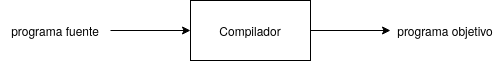
\includegraphics[scale=0.5]{Compilador.png}
\caption{Un compilador}
\label{Compilador}
\end{figure}

Un lenguaje de programación es una notación para describir computaciones a personas y a máquinas.
Pero para que un programa sea ejecutable, antes debe ser traducido a un formato comprensible para una máquina.
Los sistemas de software que se encargan de esta traducción son denominados \textit{compiladores}.
De forma simple, un compilador es un programa que puede leer un programa especificado en un \textit{lenguaje fuente} y traducirlo en un programa equivalente en un \textit{lenguaje objetivo}.
En la imagen~\ref{Compilador} se puede observar un esquema simplificado de esta idea.

Un intérprete es otra clase común de procesador de lenguajes.
En lugar de producir un programa objetivo como resultado de una traducción, un intérprete simula ejecutar directamente las operaciones especificadas en el programa fuente, en base a las entradas suministradas por el usuario y retornando las salidas producidas como resultado de la ejecución.
En la figura~\ref{Intérprete} se puede apreciar la diferencia esencial entre ambas clases de procesadores de lenguajes.

\begin{figure}[h]
\centering
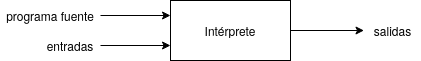
\includegraphics[scale=0.5]{Interprete.png}
\caption{Un intérprete}
\label{Intérprete}
\end{figure}

Si entramos un poco más en detalle, podemos observar que el proceso de transformación está compuesto por dos etapas: \textit{análisis} y \textit{síntesis}.
En el caso de la primera etapa, su desarrollo puede realizarse de manera idéntica tanto para compiladores como para intérpretes.
En cambio, la segunda presenta diferencias sustanciales entre ambos.
Debido que nuestro objetivo es implementar un intérprete para el lenguaje, nos concentraremos solo en el estudio de este.

\subsection{Análisis}

La parte del análisis divide el programa fuente en distintas piezas e impone una estructura gramatical a las mismas.
Luego, utiliza esta estructura para crear una representación intermedia del programa fuente.
Si la etapa de análisis detecta que el programa presenta errores sintácticos o incoherencias semánticas, entonces deberá proveer mensajes informativos para que el usuario pueda aplicar las correcciones adecuadas.
En nuestro caso, la representación intermedia que utilizaremos serán los \textit{arboles de sintaxis abstracta}.
La transformación del programa fuente a nuestra representación intermedia, no es trivial.
Para facilitar la misma, comúnmente se divide esta tarea en varias fases.

\subsubsection{Análisis Léxico}

En esta etapa, también llamada \textit{fase de escaneo}, se analiza la entrada carácter por carácter y se divide la misma en una serie de unidades elementales denominadas \textit{componentes léxicos}.
Por cada componente léxico, la fase de escaneo produce como salida un \textit{token} que pertenece a cierta categoría gramatical y posee una cantidad determinada de atributos con información relevante para las siguientes fases de análisis.
En esta etapa, además, se filtran elementos como los espacios en blanco y los comentarios.

\subsubsection{Análisis Sintáctico}

Esta es la fase que comúnmente se denomina \textit{parser}.
El parser utiliza los tokens obtenidos en la etapa previa, para crear una representación intermedia de la estructura gramatical del flujo total de tokens.
Como mencionamos anteriormente, nosotros utilizaremos un \textit{árbol de sintaxis abstracta} como representación.
Las fases posteriores del intérprete emplearán esta estructura gramatical para continuar el análisis del programa fuente.

\subsubsection{Análisis Semántico}

La última etapa del análisis es la de \textit{chequeos estáticos}.
La misma se encarga de verificar si las restricciones semánticas impuestas en la definición del lenguaje son respetadas.
Una parte importante de este análisis es el llamado chequeo de tipos (\textit{typecheck}).
Comúnmente, esta fase toma como entrada la representación intermedia obtenida en la etapa previa, y le agrega las anotaciones de tipos adecuadas, necesarias para continuar el análisis en etapas posteriores.

\subsection{Síntesis}

La parte de síntesis de un compilador es muy diferente a la de un intérprete.
Para el primero, tenemos que construir el programa objetivo utilizando la representación intermedia, junto con toda la información adicional recopilada en las etapas previas.
Habitualmente, esta fase se divide en otras dos partes, la \textit{generación de código intermedio} y la \textit{generación de código objeto}.
En la \textit{generación de código intermedio} se obtiene una representación independiente de la máquina, pero fácilmente traducible a lenguaje ensamblador.
En cambio, la \textit{generación de código objeto} es totalmente dependiente de la arquitectura concreta para la que se esté desarrollando el compilador.
Adicionalmente, durante estas fases comúnmente se aplica algún proceso de optimización sobre el código generado.

Del otro lado, como el objetivo de un intérprete difiere con el de un compilador, sus etapas de síntesis también lo hacen en la misma manera.
Para obtener los resultados del programa, debemos partir del \textit{árbol de sintaxis abstracta} obtenido luego de la fase de \textit{análisis} del intérprete y, junto con los datos de entrada sustentados por el usuario, simular la ejecución del programa en base a las acciones especificadas en el código del mismo.
De esta forma, una vez finalizada la ejecución, se obtienen las salidas del programa.
En la imagen~\ref{Fases} se puede observar la estructura de nuestro intérprete.

\begin{figure}[h]
\centering
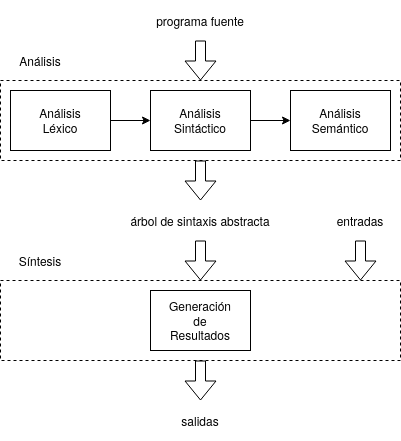
\includegraphics[scale=0.5]{Fases.png}
\caption{Estructura de un intérprete}
\label{Fases}
\end{figure}

% Ideas!!
\iffalse

% cosas que faltan
* Manejo de errores y excepciones
* canales de input y output

% concepto
Introducción: Presentar lo que estamos haciendo, es decir, contar que hay un lenguaje definido informal e incompletamente con el que se enseña una materia. Presentar ejemplos de todo lo que se hace con el lenguaje. Como si se lo contaras a alguien que sabe de programación pero no cursó la materia.
Contaríamos también qué cosas NO están bien definidas, qué ambigüedades encontramos, etc

% idea
la idea que tengo es que en la introducción hablamos de las características del lenguaje, y de lo que se enseña en la materia con él
pero no hablamos del lenguaje en particular
o sea, podemos dar algún ejemplo
pero no es que presentamos "el lenguaje tiene estas instrucciones: blablabl"
sino que decimos que es un lenguaje imperativo, que tiene manejo de memoria, etcétera
mencionamos todas las características
pero no damos formalmente nada
en el primer capítulo sí presentaríamos más detalladamente el lenguaje, como un tutorial
(el lenguaje nuestro, ya bien definido)
(pero no formalmente, sino como tutorial)
o sea, luego de leer la introducción, el lector tiene que saber de qué se trata el lenguaje, qué características tiene (o queremos que tenga), que cosas NO tiene
(y no va a tener)
pero no es que leyendo la intro lo vaya a aprender a usar
cuando lea el primer capítulo sí ya puede programar
a partir del capítulo 2 ya sería algo técnico
de cómo lo implementamos

% finalidad
incluida la finalidad con respecto a la materia también

% motivación
o sea, lo que yo dije es medio breve
me parece bueno que primero esté la motivación
¿por qué otro lenguaje?
o sea, no es que estamos definiendo un lenguaje imperativo porque tenemos ganas
sino que hay un motivo inicial
y es didáctico
así que sí, hay que hablar de la materia y de los conceptos que se enseñan con este lenguaje (que son muchísimos)

% estructura
o sea imagino de mínima:
Intro:
* Motivación
* Características del lenguaje
* Organización general de la tesis

% diferencias
pero no se pretende que alguien lea la intro y pueda programar
se pretende que alguien entienda por qué queremos implementar este lenguaje, y qué características tiene

% características
deberíamos hablar de tipado, de polimorfismo, de encapsulamiento
deberíamos hablar de manejo de memoria
de qué conceptos se enseñan en la materia
\fi